\documentclass[12pt]{article}
\usepackage{graphicx} % Required for inserting images
\usepackage{subfig}
\usepackage[spanish, es-tabla]{babel}
\usepackage[utf8]{inputenc}
\usepackage{amsmath}
\usepackage{multirow}
\usepackage[table,xcdraw]{xcolor}
\usepackage[colorlinks=true, linkcolor=black, urlcolor=blue]{hyperref} 
\usepackage{geometry}
\newgeometry{bottom=3cm, top=3cm, left=3cm, right=3cm}
\usepackage{fancyhdr}
\providecommand{\abs}[1]{\lvert#1\rvert}
\providecommand{\norm}[1]{\lVert#1\rVert}


\usepackage[document]{ragged2e}

\begin{document}

\renewcommand{\baselinestretch}{1.5}

\begin{titlepage}
    \centering
    {\bfseries\LARGE  \par}
    \vspace{1cm}
    {\scshape\Large  \par}
    \vspace{3cm}
    {\scshape\Huge Coordenadas baricéntricas de los planetas del sistema solar
 \par}
 \vspace{10mm}
 \begin{figure}[!h]
    \centering
    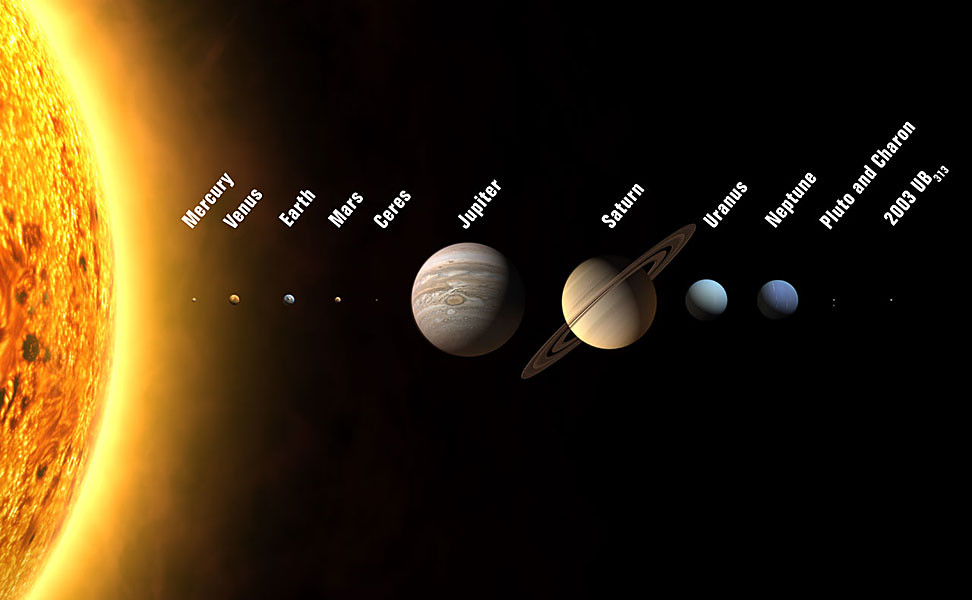
\includegraphics[scale=0.5]{sistema.png}
\end{figure}
    \vspace{3cm}
    {\itshape\Large  \par}
    \vfill
    {\Large Autor: \par}
    {\Large Eduardo Pérez del Castillo\par}
    \vfill
    {\Large Junio 2024 \par}

\end{titlepage}

\newpage

\section{Objetivos}
El objetivo de este documento es aprender un poco sobre que son
y que representan las coordenadas baricéntricas de los planetas del sistema
solar. Asimismo, haremos un pequeño análisis de unas simulaciones hechas. Además, aprenderemos
a usar de manera muy superficial la librería \textit{astropy}.


\section{Intruducción}
Las coordenadas baricéntricas, como cualquier sistema de coordenadas, tiene
un origen (baricentro). Se utiliza para describir la posición de un objeto en
relación con el centro de masa de un sistema de cuerpos. 
En este caso en concreto, el centro de masas de nuestro sistema (el sistema solar) 
para muchos, podría tratarse del Sol. Sin embargo, esto es una
idea errónea. El centro de masas de nuetro sistema se encuentra 
ligeramente desplazado de la posición de la estrella central. 

\vspace{5mm}

Como el sistema solar es un sistema discreto, podemos decir que:

\begin{equation}
    R_{CM}=\frac{\sum_i m_ir_i}{\sum_i m_i}
    \label{eq1}
\end{equation}

Hagamos los cálculos con Júpiter, por ejemplo. Dicho planeta dista del Sol una 
distancia $r =  778.330.000 km$, con una masa de $M_J = 1,899 \cdot 10^{27} kg$.
El sol tiene una masa de $M_S = 1,989 \cdot 10^{30} kg$ y radio de $R_S = 696.000 km$.
El centro de masas del Sol ($x$) cumplirá que:

\begin{center}
    $M_s \cdot x = M_J *\cdot(r-x)$
\end{center}

y despejando $x$:

\begin{equation}
    x = \frac{M_J}{M_s + M_j}r
\end{equation}

Sustituyendo obtenemos:

\begin{center}
    $x = 742403 km$
\end{center}

Es decir, en el sistema Sol-Júpiter el centro de masas estará a $742403 - R_S = 46403 km$ de la superficie solar.

\newpage


\section{Análisis del programa}
Antes de pasar con el análisis del programa, se dejará un pequeño vocabulario
de apoyo.

\begin{itemize}
    \item \textbf{Efemérides}: las efemérides son tablas de datos o bases de datos que detallan las posiciones
    de los cuerpos celestes en momentos en específicos.
    \item \textbf{Baricentro}: el baricentro del sistema solar es el centro de masa común alrededor del cual todos 
    los cuerpos del sistema solar orbitan. No está exactamente en el centro del Sol, 
    sino que se mueve en función de la posición y masa de los planetas, 
    lunas y otros objetos del sistema solar.
\end{itemize}


\subsection{Librerías}

\begin{figure}[!h]
    \centering
    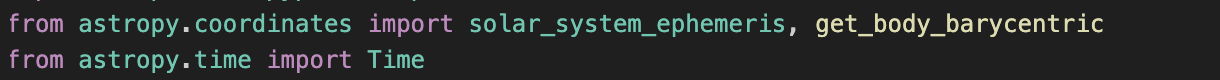
\includegraphics[scale=0.6]{librerias.png}
    \caption{Librería Astropy}
    \label{im1}
\end{figure}
En este programa hemos usado la librería \textit{astropy}, una librería muy común y potente
en el ámbito de la astrofísica. \textit{astropy.coordinates} es un módulo dentro de la librería 
\textit{astropy}. Dicho módulo nos permite realizar cálculos relacionados con las coordenadas astronómicas.
Al escribir \textit{solar\_system\_ephemeris} estamos importando una herramienta la cual contiene las efemérides
del sistema solar. Asimismo, \textit{get\_body\_barycentric} es una función que nos devuelve 
las coordenadas baricentricas del cuerpo celeste que le indiquemos. 

\vspace{5mm}

Por otro lado, \textit{astropy.time} es un módulo de \textit{astropy} que nos permite seleccionar un tiempo
en específico en la linea temporal que nos interese.

\vspace{5mm}

Con este conjunto de librerías vamos a poder observar las efemérides de los cuerpos celestes del sistema solar 
en un espacio de tiempo determinado.

\newpage 

\subsection{Configuración de efemérides}

\begin{figure}[!h]
    \centering
    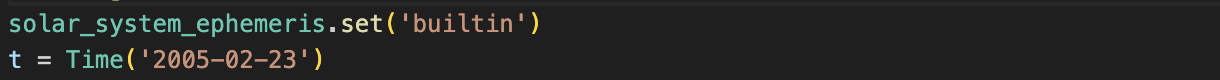
\includegraphics[scale=0.6]{efemerides.png}
    \caption{Configuración de efemérides}
    \label{im2}
\end{figure}

Ahora es necesario seleccionar las efemerides que nos interese para este problema.
Por ello, con \textit{solar\_system\_ephemeris.set('builtin')} 
podremos elegir una interfaz en la que seleccionar las efemérides que queramos. En este caso, hemos escogido \textit{builtin}. 
No es la más precisa, pero es suficiente para el objetivo de este experimento. En caso de querer usar efemérides más precisas, 
acudir a \textit{de432s} o \textit{JPL}.

\vspace{5mm}
Por otro lado, la variable $t$ ha sido definida mediante la herramienta \textit{Time} de la librería \textit{astropy}. Dicha
herramienta nos sirve para seleccionar la fecha de tiempo en la que trabajaremos con las efemérides.


\subsection{Simulaciones}
En la siguiente imagen quedarán indicadas las coordenadas baricentricas de cada planeta en el sistema solar.

\begin{figure}[!h]
    \centering
    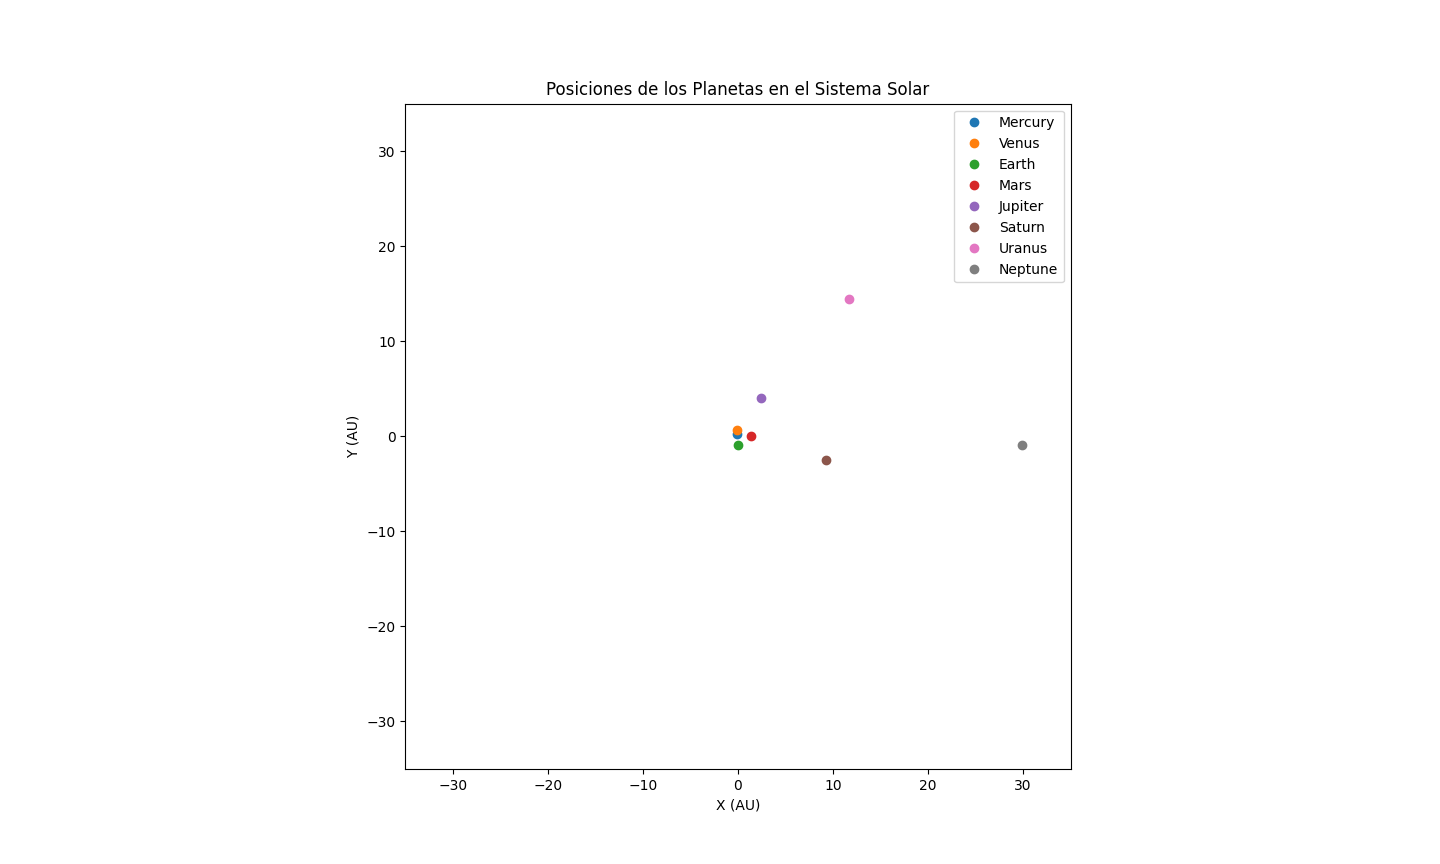
\includegraphics[scale=0.4]{2d.png}
    \caption{Representación en 2d}
    \label{im3}
\end{figure}


Haremos un pequeño calculo con Neptuno simplemente para corroborar que el método ha sido bien empleado.

\begin{figure}[!h]
    \centering
    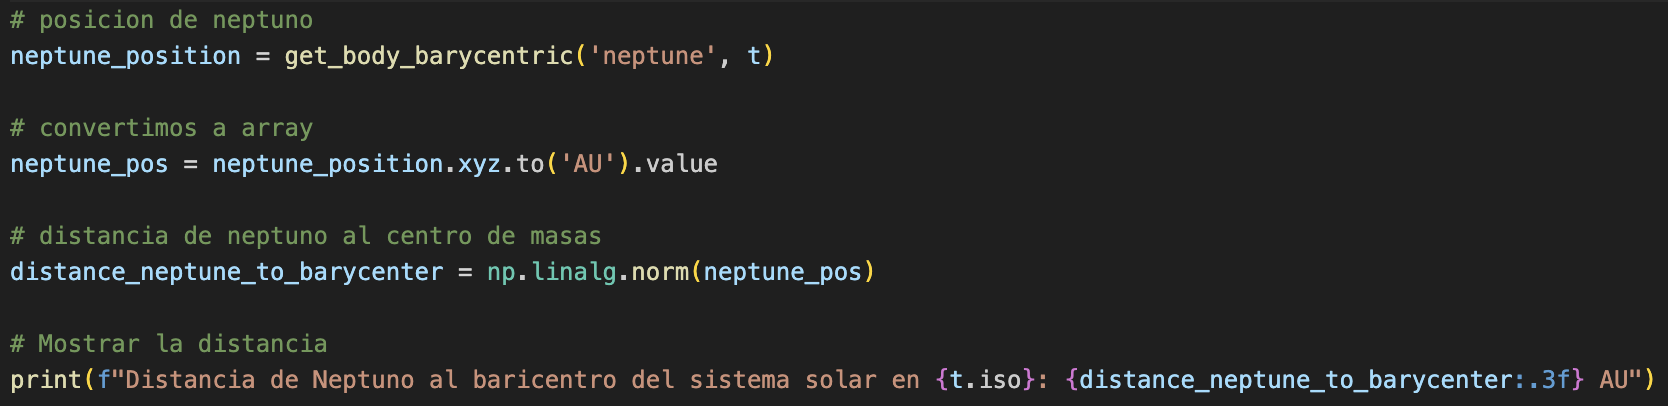
\includegraphics[scale=0.4]{codigo.png}
    \caption{Cálculo de comprobación}
    \label{im4}
\end{figure}

Lo que hemos hecho es obtener las coordenadas baricéntricas de neptuno en el tiempo que hemos especificado. Luego,
como hemos convertido esas coordenadas en un array, es decir, en un vector, hacemos la norma del mismo para obtener la
longitud (distancia de Neptuno al baricentro del sistema solar) del vector. Con esto, obtenemos una distancia de $29.893$ $AU$. 
Si nos fijamos en la figura (\ref{im3}), vemos que concuerda con lo obtenido. 

\vspace{5mm}

Dejaremos representado también una figura en tres dimensiones para hacernos una idea más realista de los resultados.
\begin{figure}[!h]
    \centering
    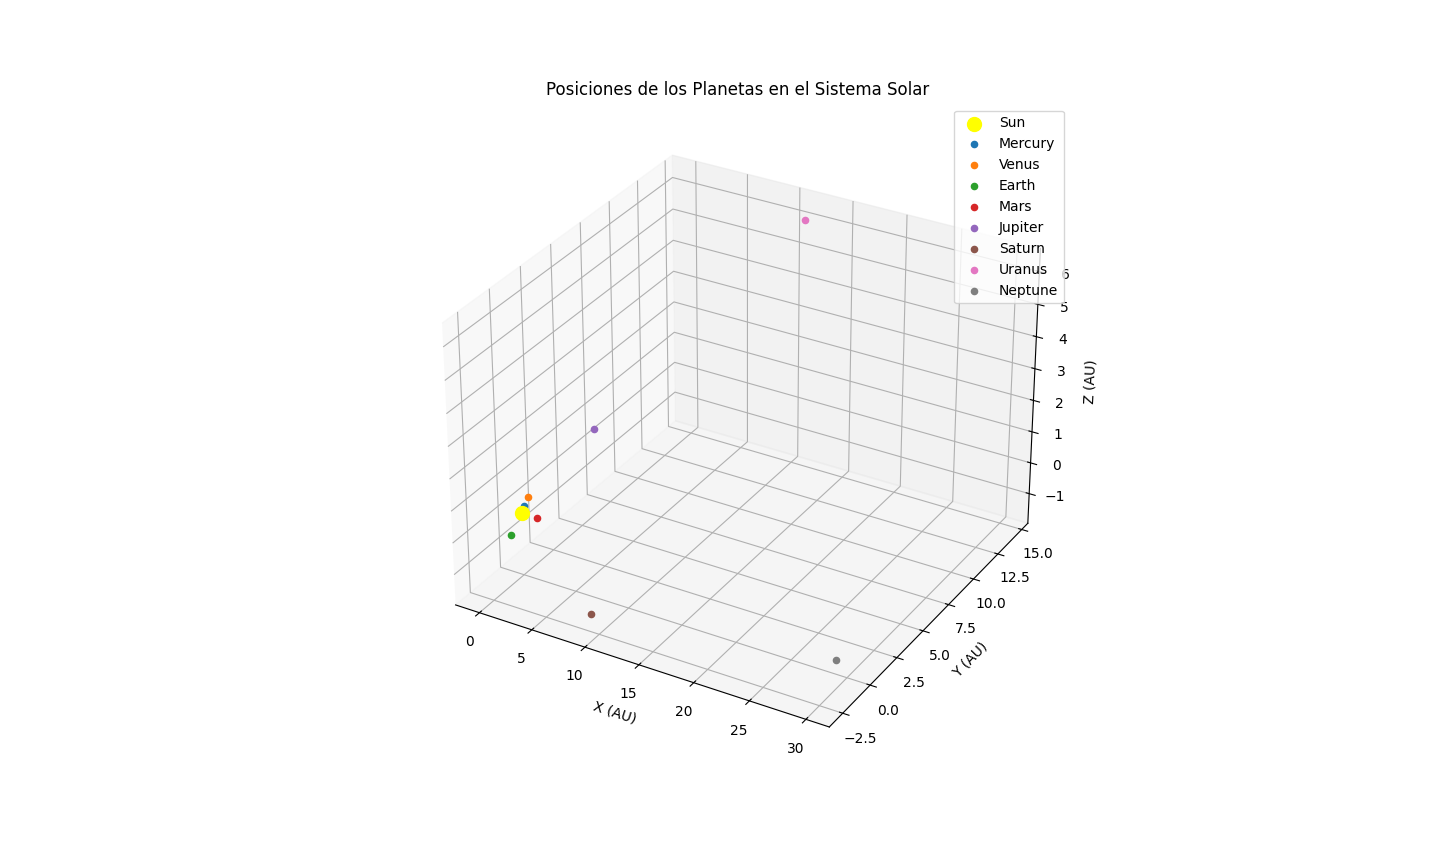
\includegraphics[scale=0.4]{3d.png}
    \caption{Representación en 3d}
    \label{im5}
\end{figure}

\newpage

\section{Conclusiones}
En este pequeño experimento hemos podido realizar una pequeña y superficial introducción a la librería \textit{astropy}. Una librería
muy útil y potente para realizar cálculos astronómicos fundamentales. Asimismo, hemos aprendido a obtener las coordenadas
baricentricas de cualquier cuerpo celeste del sistema solar. También hemos aprendido nuevos concepto como pueden ser las efemérides
o baricentro.

\newpage

\section{Bibliografía}
\begin{itemize}
    \item 
       {[1]\emph{Wikipedia, coordenadas baricéntricas (astronomía).}}
   \end{itemize}




\end{document}